\chapter{Background Knowledge}

\section{A brief overview of \gls{dms}}
In the 1980s, printers, scanners, and household computers started to gain popularity.
Organizations start to take actions on managing their information records and assets seriously.
At that time, Document Image Processing (DIP) systems are the only available software to satisfy their needs.
DIP is the electronic version of filing cabinet where documents need to be scanned, indexed, and store in the system \cite{1_adam_2008}.
DIP can also analyse figures, texts, and handwriting \cite{akram2010document} using various image processing techniques.
\begin{wrapfigure}{l}{0.5\textwidth}
	\centering
	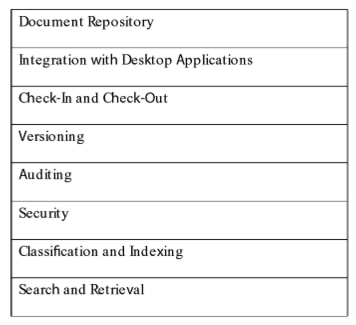
\includegraphics[scale=0.7]{res/bg-knowledge/edms-components.png}
	\caption{Basic components of EDMS \cite{1_adam_2008}}
	\label{fig:edms-components}
\end{wrapfigure}
Later on in the 1990s, Electronics Document Management System (EDMS) is developed targeting large enterprises with high volume of documents.
It is the improved version of DIP with workflow functionality.
Workflow functionality enables organizations to passed around scanned document throughout the organization to designated employee.
EDMS also has its own document repository allowing documents to be indexed and tracked using version control.
There are various sub-types of EDMS such as Electronic Record Management Systems (ERMS) deals mainly with record keeping.
Enterprise Content Management (ECM), suites of applications, deals with document and record management.
Nowadays, EDMS acronym is shortened to DMS.
Figure \ref{fig:edms-components} shows a basic components of DMS.
Most DMS applications have these components implemented within.
\begin{description}
	\item[Document Repository] \hfill \\
	A place where indexed documents are stored.
	Typically on a hard disk of a network server.
	\item[Integration with desktop applications] \hfill \\
	Allowing user to save documents straight to application when document is created.
	It is usually a 3rd party add-on embedded in popular office applications such as Microsoft Office.
	\item[Check-in and check-out] \hfill \\
	This feature controls who is allowed to make changes or to read documents.
	Basically, it is a user permission control system.
	\item[Versioning] \hfill \\
	Keeping track of changes by assigning a version number to a document.
	The number is incremented after the document passes major revisions.
	User can access the previous versions of the document.
	\item[Auditing] \hfill \\
	Track who changes document, when, and where.
	Only authorized user can read these information.
	\item[Security] \hfill \\
	Controls how documents should be stored in the server to prevent hackers from attacking the system.
	\item[Classification and indexing] \hfill \\
	Metadata and tags provide more information to documents.
	It helps to search and retrieve documents easier.
	\item[Search and Retrieval] \hfill \\
	Allow user to retrieve documents according to keywords.
	Keywords can be a metadata or contents within a document.
	A system may offer advance search criteria by looking for individual fields and combine with other fields using basic logical operations (AND, OR, NOT). 
\end{description}